% !TeX root = ../build/main.tex

Citadel is a self-sovereign identity (SSI) protocol built on tope of Dusk that allows users of a given service to manage their digital identities in a fully transparent manner. More specifically, every user can know which information about them is shared with other parties, and accept or deny any request for personal information.

\subsection{Properties}

With Citadel, users of a service can request licenses that represent their \emph{right} to use such a service. Citadel satisfies the following properties:

\begin{itemize}
	\item \emph{Proof of ownership}: users can prove that they own a valid license that allows them to use a certain service.
	\item \emph{Proof of validity}: users with a valid license can prove that their license has not been revoked and is valid.
	\item \emph{Unlinkability}: different services used by a same user cannot be linked from one another.
	\item \emph{Decentralized session opening}: when users start using a service, the network learns that this happened and the license used to access to the service cannot be used again.
	\item \emph{Attribute blinding}: users have the power to decide exactly what information they want to share and with whom.
\end{itemize}

\subsection{The parties involved}

Citadel involves three (potentially different) parties:

\begin{itemize}
    \item The \emph{user} is the person who interacts with the wallet and requests licenses in order to claim their right to make use of services.
    \item The \emph{service provider} (SP) is the entity that offers a service to users. Upon verification that a service request from a user is correct, it provides such service.
    \item The \emph{license provider} (LP) is the entity that receives requests for licenses from users, and upon acceptance, issues them. The LP can be the same SP entity or a different one.
\end{itemize}

\subsection{The elements involved}

Below there is the list of the elements involved in the protocol. The details of their structure and their role are explained in the following sections. 

\begin{itemize}
	\item A \emph{request} is a set of information that the user sends to the network in order to inform the LP that they are requesting a license. It includes an stealth address where the license will be sent to.
	\item A \emph{license} is an asset that represents the right of a user to use a certain service. In particular, a license contains a set of attributes that are associated to the requirements needed to make use of that service.
	\item The \emph{LicenseProverParameters} are the set of parameters needed by the user to compute a proof that proves their license ownership.
	\item A \emph{session} is a set of public values sent by the user to the network that are associated with the initiation of the use of a service.
	\item A \emph{session cookie} is a set of values that allow {\color{red}[who?]} to verify that a session was opened correctly.
\end{itemize}

\subsection{Protocol flow}

{\color{red}[Missing explanation]}

\begin{figure}[h]
	\centering
	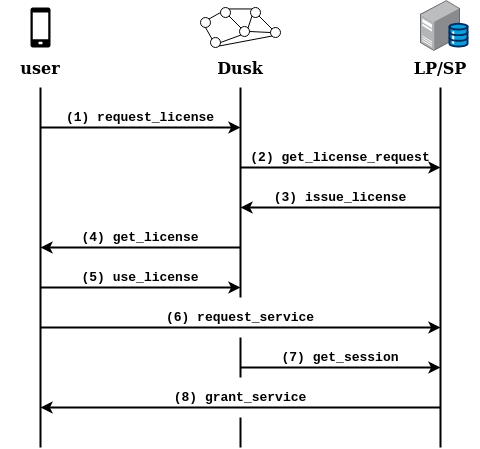
\includegraphics[width=.4\textwidth]{\figs/protocol.png}
	\caption{Overview of the protocol messages exchanged between the user, Dusk's network, and the LP/SP.}
	\label{fig:protocol}
\end{figure}

